\section{Marco Teórico}

\subsection{Circuitos Magnéticos}
Un circuito magnético está compuesto por un material ferromagnético que confina el flujo magnético. La relación entre la fuerza magnetomotriz (FMM), el flujo magnético ($\phi$) y la reluctancia ($\mathcal{R}$) está dada por:

\begin{equation}
    \mathcal{F} = N I = \phi \cdot \mathcal{R}
\end{equation}

donde $N$ es el número de espiras, $I$ la corriente y $\mathcal{R}$ la reluctancia del circuito:

\begin{equation}
    \mathcal{R} = \frac{l}{\mu A}
\end{equation}

con $l$ la longitud media del núcleo, $A$ el área transversal y $\mu$ la permeabilidad del material.

\subsection{Curva B-H y Ciclo de Histéresis}
La relación entre la densidad de flujo magnético $B$ y la intensidad de campo magnético $H$ en un material ferromagnético no es lineal. Al someter el material a un ciclo completo de magnetización, se obtiene el ciclo de histéresis (Figura 1).

\begin{figure}[h]
\centering
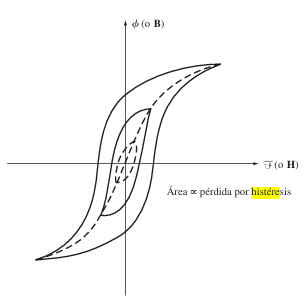
\includegraphics[width=0.6\textwidth]{figures/figura-ciclo-histeresis.png}
\caption{Ciclo de histéresis típico de un material ferromagnético.}
\label{fig:histeresis}
\end{figure}

Parámetros característicos:
\begin{itemize}
    \item $B_{\text{sat}}$: Inducción de saturación
    \item $B_r$: Inducción remanente (cuando $H = 0$)
    \item $H_c$: Campo coercitivo (cuando $B = 0$)
\end{itemize}

Como se ha visto, para cambiar la orientación de los dominios magnéticos se requiere energía, lo que origina pérdidas en todas las máquinas y transformadores. Las pérdidas por histéresis en el núcleo de hierro corresponden a la energía necesaria para reorientar los dominios durante cada ciclo de corriente alterna aplicada al núcleo. El área comprendida dentro del ciclo de histéresis es directamente proporcional a la energía perdida por ciclo. Cuanto menores sean las variaciones de la fuerza magnetomotriz aplicada al núcleo, menor será el área del ciclo y, por tanto, menores serán las pérdidas resultantes~\cite{chapman}.

\subsection{Pérdidas en el Núcleo}
Las pérdidas totales en un núcleo ferromagnético sometido a un campo alterno son:

\begin{equation}
    P_{\text{núcleo}} = P_h + P_f
\end{equation}

\textbf{Pérdidas por histéresis} ($P_h$): proporcionales al área del ciclo de histéresis y a la frecuencia:

\begin{equation}
    P_h = K_h \cdot f \cdot B_{\text{máx}}^n
\end{equation}

donde $K_h$ es una constante del material, $f$ la frecuencia, $B_{\text{máx}}$ la inducción máxima y $n$ el exponente de Steinmetz (usualmente $n \approx 1.6$ a $2.0$).

\textbf{Pérdidas por corrientes parásitas} ($P_f$): un flujo variable en el tiempo induce voltajes en el núcleo ferromagnético, generando corrientes circulantes (corrientes de remolino o parásitas) que disipan energía en forma de calor~\cite{chapman}. La magnitud de estas pérdidas depende del tamaño de los remolinos y de la resistividad del material. Para reducirlas se emplean dos métodos:

\begin{itemize}
    \item \textbf{Laminación del núcleo:} dividir el núcleo en finas láminas aisladas entre sí limita el tamaño de los remolinos, reduciendo el voltaje inducido y las pérdidas asociadas.
    \item \textbf{Aleaciones de alta resistividad:} agregar silicio al acero del núcleo aumenta su resistividad, disminuyendo la corriente inducida para un flujo dado.
\end{itemize}

La combinación de ambos métodos puede reducir las pérdidas por corrientes parásitas hasta hacerlas mucho menores que las pérdidas por histéresis:

\begin{equation}
    P_f = K_f \cdot f^2 \cdot B_{\text{máx}}^2
\end{equation}
